% % % % header removed
%\section{Methodology}


The methodology is divided into two components: Synthesis of the feature vector using tensorization (Section~\ref{sec:tensor}) and classification using an ANN (Section~\ref{sec:ANN}). 
%\subsection{Tensorization Framework for Combination of Multi-frequency Data}
\subsection{Data Preprocessing}
\label{sec:tensor}
A tensorization framework is proposed which utilizes the Kronecker product of two matrices $\mathbf{A} \in \mathbb{F}^{p\times q}$ and $\mathbf{B} \in \mathbb{F}^{r \times s}$ denoted as $\mathbf{A} \otimes \mathbf{B}$ and is defined as, 
%
\begin{equation} 
\mathbf{A} \otimes \mathbf{B} = \left[\begin{array}{rrrr}
a_{11} \mathbf{B}  & a_{12}\mathbf{B}  & \dots  & a_{1q} \mathbf{B}\\
\vdots  & \vdots   & \ddots   & \vdots\\
a_{p1} \mathbf{B} & a_{p2}\mathbf{B} & \dots & a_{pq} \mathbf{B}      
\end{array}\right]_{pr \times qs}
\end{equation}  
%
where $\mathbb{F}$ is a field such as $\mathbb{R}$ or $\mathbb{C}$. The matrix block  $a_{ij}\mathbf{B}$ is of dimension of $\mathbf{B}$.
In general, the Kronecker product of two matrices is non-commutative, meaning that $\mathbf{A}\otimes \mathbf{B} \ne \mathbf{B}\otimes \mathbf{A}$. Each entry of $\mathbf{A} \otimes \mathbf{B}$ (or $\mathbf{B}\otimes \mathbf{A}$) is of the form $a_{ij}b_{kl}$ (or $b_{kl}a_{ij}$). Thus $\mathbf{B}\otimes \mathbf{A}$ can be obtained by permuting the entries of $\mathbf{A}\otimes \mathbf{B}$.

In PolSAR literature, the Kronecker product is used to derive the Kennaugh matrix from the scattering matrix $  \mathbf{S} $.  
A radar target is characterized by a scattering matrix $\mathbf{S}$ which describes the dependence of scattering properties on polarization. It is defined in the $hv$ basis as,
%Current technology allows for simultaneous multi-band (C, L, P) acquisition of PolSAR data of the same scene using airborne sensors. Thus efficient techniques for augmentation and fusion of the acquired data for analysis is required. 
%This may be mitigated by use of the Kronecker product, for relevant parameters from the PolSAR images corresponding to individual bands such as the roll invariant parameters. 
%The generation of the input feature 
%The tensorized feature vector is generated as follows. 
\begin{equation}
\bm{\mathbf{S}} =
  \begin{bmatrix}
    S_{hh} & S_{hv}  \\
    S_{vh} & S_{vv}
  \end{bmatrix}
 \label{eqn:scattring}
\end{equation}
where each element is a complex quantity composed of the amplitude and the phase of the scattered electromagnetic signal.
The Pauli target vector is generated from $\mathbf{S}$ as,
\begin{equation}
\bm{k_p} = \frac{1}{\sqrt{2}} \left[ S_{hh}+S_{vv} \quad S_{hh}-S_{vv} \quad  2S_{hv} \right] ^{T}
\end{equation}
%\begin{equation}
%	[T] =  \bm{k} . \bm{k}^{*T} 
%\end{equation}
which is then utilized to obtain the coherency matrix, $\mathbf{T}$, by spatial ensemble averaging,
\begin{equation}
\mathbf{T} = \frac{1}{N} \sum_{i=1}^{N} \bm{k_{p_i}}\bm{k_{p_i}}^{\dagger} 
\end{equation}
where $\dagger$ is the conjugate transpose. The coherency matrix $\mathbf{T}$ is a hermitian positive semi-definite matrix, and thus  can be diagonalized as,
\begin{equation}
\mathbf{T}  = \mathbf{U}  \mathbf{ \Lambda }\mathbf{ U^{\dagger}} = \sum\limits_{i=1}^{3}\lambda_{i}\bm{u_i} \bm{u_i}^{\dagger}
\end{equation}
where $\mathbf{ \Lambda}$ is a $3\times3$ diagonal matrix with non-negative real eigenvalues, and $\mathbf{U} = [\bm{u_1}\ \bm{u_2}\ \bm{u_3}]$ is a unitary matrix of the SU(3) group, where $\bm{u_1}$, $\bm{u_2}$, and $\bm{u_3}$ are the orthogonal eigenvectors corresponding to the eigen values $\lambda_1,\lambda_2,\lambda_3$. 
%$F = \{f_1, f_2 \ldots f_k\}$ are the frequency bands with $k$ being the number of bands.

If $ \mathbf{T}_{1} = \mathbf{U_1}\mathbf{\Lambda_1}\mathbf{U_1^\dagger}$ and $ \ \mathbf{T}_{2} = \mathbf{U_2}\mathbf{\Lambda_2}\mathbf{U_2^\dagger}$ are the eigenvalue/eigenvector decompositions of $\mathbf{T}_{1}$ and $\mathbf{T}_{2}$ respectively, then,
\begin{equation}
\mathbf{T}_{1}\otimes\mathbf{T}_{2}=(\mathbf{U_1}\otimes \mathbf{U_2})(\mathbf{\Lambda_1}\otimes\mathbf{\Lambda_2})(\mathbf{U_1}\otimes \mathbf{U_2})^{\dagger}
\end{equation}
is the eigen decomposition of $\mathbf{T}_{1}\otimes\mathbf{T}_{2}$ utilizing the mixed Kronecker product properties. Here $\mathbf{T_k}$ corresponds to the frequency band $f_k$.  
%In this study, $f_k \in \{C,\ L,\ P\}$ bands.
Hence, using the Kronecker product the diagonal matrices corresponding to two or more frequencies may be combined to obtain the tensorized product, 
\begin{equation}
\mathbf{X}_{f_1, f_2, \ldots ,f_k}  =  \Lambda_{f_1} \otimes \Lambda_{f_2} \otimes \ldots \otimes {\Lambda_{f_k}}.
\end{equation}
% In this study, $F \in \{C,\ L,\ P\}$ bands. 
%\begin{equation}
%W_{f_1 f_2} = \vect{\lambda_{f_1}} \otimes \vect{\lambda_{f_2}} \otimes \ldots \otimes %\vect{\lambda_{f_k}}
%\end{equation}
%Let $\bm{A} = \left( a_{ij} \right)_{n\times n}$ and $\bm{B} = \left( b_{ij} \right)_{n\times n}$. The Kronecker product is defined with the operator $\otimes$ as,
%\begin{align}
%\nonumber \bm{A} \otimes \bm{B} &= \left(a_{ij}\bm{B}\right)_{n^2\times n^2} \\ 
%&=   \begin{bmatrix}
%    a_{11}\bm{B} & a_{12}\bm{B} & \ldots & a_{1n}\bm{B}  \\
%    \vdots &  \ddots & & \vdots \\
%    a_{n1}\bm{B} & a_{n2}\bm{B} & \ldots & a_{nn}\bm{B}  \\
%  \end{bmatrix}
%\end{align}
The non-zero elements of the matrix $\mathbf{X}_{f_1, f_2, \ldots ,f_k}$ is used as input vector $\bm{x}$ in the  ANN. The eigen decomposition of the Kronecker product of the coherency matrices corresponding to C-, L- and P-band is used to generate feature vectors for classification. 

Current technology allows for simultaneous multi-frequency acquisition of PolSAR data of the same scene. Thus, efficient techniques for augmentation and fusion of the acquired data for the analysis of enhanced information content is desirable. The proposed tensorization framework allows for homogeneous composition of information from each frequency-band and prevents an \emph{a-priori} bias towards a dominant band. Hence, such a combination leads to a higher dimensional representation which, in general, is more separable for classification tasks if exploited by suitable learning algorithms. 

%In the proposed ANN algorithm, this increased dimensionality is leveraged for accurate classification in a computationally efficient manner.

%In general, higher dimensional data is more separable during classification tasks. However, due to computational complexity associated with the processing of these datasets, suitable steps are applied to minimize the dimensionality. 
%In contrast, the proposed ANN algorithm leverages this increased dimensionality in a computationally efficient manner. 

%$viz.\ W_{CL} = \vect{\lambda_{C}} \otimes \vect{\lambda_{L}}.
%outline
%1- alternative way of augmenting data
%
%2- higher dimension improves seperability of classes
%
%3- so far we find compressed representation because of limitations of ML algorithms
%
%4- novel algorithm to leverage increased dimensionality
%
%5- kronecker has been used in kennaugh SxS extending to coh and cov
%
%6- bands are well and evenly mixed so that they are not understressed 





\begin{figure}[tbp] 
	\centering
	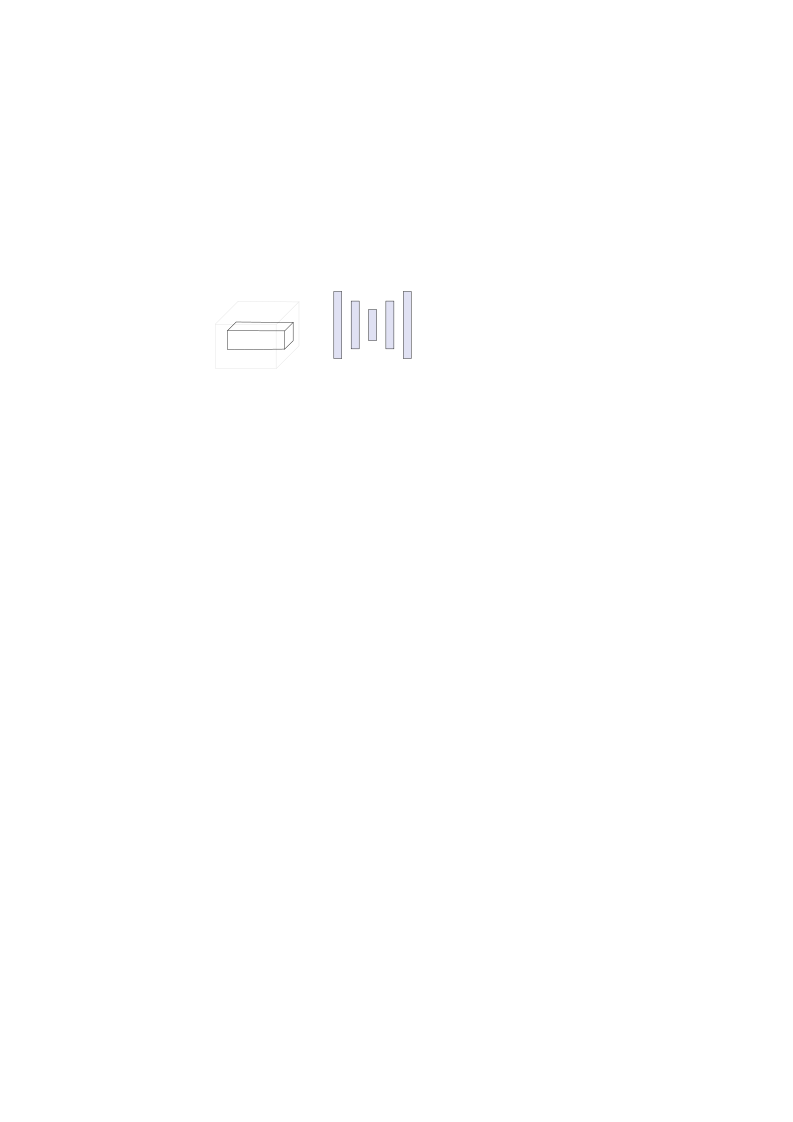
\includegraphics[width=0.95\textwidth]{Figures/Kron/AE}
	\caption{Schematic diagram of the proposed framework.}
	\label{fig:ANN}
\end{figure}

%\subsection{Unsupervised Feature Extraction using a Stochastic Sampling Stacked Auto-Encoder Network}
\subsection[Unsupervised Representation Learning using Auto-Encoders]{Unsupervised Representation Learning using \\ Auto-Encoders}

\label{sec:ANN}
The ANN architecture used in this work is divided into two stages as shown in Figure~\ref{fig:ANN}. 
First, an unsupervised stochastic sampling sparse stacked Auto-Encoder (AE) stage learns an efficient intermediate representation of the combined multi-frequency features. Subsequently, this learned representation is classified by a FF network. 
%The ANN is divided in two stages. 
%An auto-encoder structure is used to learn unsupervised %representation
%Classified by a Deep feed forward network in a fine tuning step

% Describe the AE
The AE is a  fully connected, feed-forward, non-recurrent neural network with multiple hidden layers. 
The number of nodes in the input and output layers is equal. It consists of three parts: the encoder, the decoder and a representational layer ($\bm{z}$) as shown in Figure~\ref{fig:ANN}. During the training phase, the output nodes $\bm{x_i'}$ are connected to the input nodes $\bm{x_i}$. For each pixel $i$, the AE attempts to reconstruct the  $\bm{x_i}$ as  $\bm{x_i'}$. The reconstruction error is computed and minimized over multiple iterations in order to learn an optimal reconstruction. 

% Stochastic sampling and why to use it
The AE is preceded by a  stochastic sampling block which randomly selects a vector as $\bm{x_i}$ from a $N\times N$ window in each iteration as input vector and target while training the network. This is akin to using a smoothing filter and leads to  %, which is drawn from the actual speckle statistics of the SAR image. 
improved generalization performance of the AE in the presence of speckle~\cite{zeiler2013stochastic}.
%This leads to a suppression of speckle by ensemble averaging as a part of the classification process, rather than an explicit application of SAR filtering as a pre-processing step. 
Additionally, the windows are also chosen in random order to prevent the AE from memorizing the order of input. 



This representation is built in an unsupervised manner for each pixel in the dataset. The fundamental computational unit of an AE is a connected neuron that takes as input $\bm{x_i} = \left[ x_1, x_2, \ldots ,x_n \right]$ and a bias intercept term $b$ and produces the hypothesis $h = \mathbf{s}(\sum_{i=0}^{n} \mathbf{W_{r_i}} \bm{x_i} + b)$, where $\mathbf{s}$ is a non-saturating non-linearity called  Parametric Rectified Linear Unit (PReLU). 
%More about PReLU----------
The response of $\mathbf{s}(y_i)=y_i$ when $y_i>0$ and $\mathbf{s}(y_i)=a_iy_i$ when $y_i<0$. Here, $a_i$ is a learnable parameter controlling the slope of the negative response of the PReLU~\cite{he2015delving}. 
%When $a_i = 0$ the PReLU reduces to a regular Rectified Linear Unit (ReLU).
% The PReLU can not be computed in-place like the ReLU and thus requires more computer memory, however it performs better
As the width of the input vector increases with the tensorial combination of multiple frequencies, the ReLUs tend to have difficulties with zero gradients during back-propagation. This prevents  efficient training of the AE. Hence, the use of PReLUs helps to overcome this problem and improve the convergence rate of the network.   

%how does the AE help summarize the different frequencies
The representation $\bm{x}$ has relatively high dimensionality with redundancies.
This makes classification difficult, which either leads to poor performance or requires a more complex classification scheme. However, an optimal representation learned by the AE simplifies the classification. It is observed that even with a relatively simple FF network, a high level of accuracy is obtained.  
% what happens after training? Be concise but clear
%The AE consists of three sections, encoder, representational layer ($Z$) and decoder. 
 
On completion of the training phase, the update of weights in the AE are suspended, and the decoder is disconnected. 
%The data $\bm{x}$ is applied for each pixel $i$ sequentially, and the output of learned representation layer $\bm{z_i}$ is extracted and used as input in the FF network stage. 
The representation $\bm{z_i}$ is extracted for each pixel $i$ and is used as input in the FF network stage. 

%\subsection{Classification using Feed Forward Network}
\subsection{Supervised Classification}
% finetuning or classification..?
The final classification is performed in a supervised manner by the FF network. During this stage, only the labeled training pixels are considered. $\bm{z_i}$ is applied as an input to the FF network and the labels $L_i$ are applied at the output. The error between the predicted and actual labels is minimized over multiple iterations with only the weights of the FF network being updated while utilizing the representation learned in the training phase from the AE. The terminal layer of the FF uses Softmax saturating non-linearities scaled in the range $[0,1]$, instead of PReLU. Here a value close to 1 indicates an active response to the corresponding label, while 0 represents an inactive one.  


% % % % % % % % Confidence
%Likehood based misclassification supression - remove non confidence pixels.
%avarage Confidence table?
The proposed architecture allows computation of classification confidence for each pixel as a part of the FF network. The number of nodes in the output layer is chosen to be one more than the minimum required to represent every class. This node, called zero (or null) label, remains unmapped to any label and allows the estimation of uncertainty of classification.
%To this end, a node corresponding to the zero label is added in addition to the minimum required to represent every label present in the data. This allows the estimation of uncertainty of classification.
%The output layer of the FF has one more node than the minimum number required to fully represent every label present in the training set. 
The null label represents those data points which have not been successfully classified into one of the given set of labels.
This is used to estimate the overall confidence level of the classified output by the network and simultaneously exclude pixels with high uncertainty from the final output. 
In practice, the total labeled pixels are randomly divided into three groups, training, test and validation. The fine tuning is conducted only on the training pixels, with the test pixels used to check for over-fitting at regular intervals. The network performance is measured at the end of classification over the validation pixels. 
%Since only a portion of the labeled data is used, and only a part of the total network weights are updated, this step is called fine tuning. 

 
%Ordinarily, in denoising AEs, the noise statistics are drawn from a distribution that might not match the image statistics.  instead of drawing from a random distribution which m 
%%%%%%%%%%%%%%%%%%%%%%%%%
% smoothing -  better snr - ergodicity

%introduced noise from

%, increasing the generalization ability of the AE. 
%Stochastic sampling 
%Helps with generalization 
%Its a form of denoising which draws from the actual noise statistics of the image



% % % % % % % % % % % % % % % % % % % % % % % % % % % % % % % % % %
%A neuron is a computational unit that
%takes as input X i n = X 1 , X 2 ...X n and an intercept term
%b, and produces the output, called hypothesis, h W,b (X) =
%n
%f (W x) = f ( i=1 W i x i + b), where f : ⇒ is called
%the activation function or nonlinearity.
%Rectified Linear Unit (ReLU)
%activation function [52] can be used to overcome the saturation
%problem. The ReLU f (x) = max( , x) simply thresholds the
%data at , typically = 0. The differentiation of the function
%df
%= {1 : x > , 0 : x < } Another advantage
%is defined as dx
%is that the training time for saturating activation functions is
%larger with the gradient descent algorithm than for its non-
%saturating counterparts [53]
%in-place computation
%and requiring less computer memory. A disadvantage of ReLU
%units is that when subjected to large gradients they can update
%their weights to such a state that they can not be activated by
%subsequent inputs.